\documentclass[a4paper,14pt]{extreport} % формат документа

\usepackage{amsmath}
\usepackage{cmap} % поиск в ПДФ
\usepackage[T2A]{fontenc} % кодировка
\usepackage[utf8]{inputenc} % кодировка исходного текста
\usepackage[english,russian]{babel} % локализация и переносы
\usepackage[left = 2cm, right = 1cm, top = 2cm, bottom = 2 cm]{geometry} % поля
\usepackage{listings}
\usepackage{graphicx} % для вставки рисунков
\usepackage{amsmath}
\usepackage{float}
\usepackage{multirow}
\graphicspath{{img/}}
\DeclareGraphicsExtensions{.pdf,.png,.jpg}
\newcommand{\anonsection}[1]{\section*{#1}\addcontentsline{toc}{section}{#1}}

\lstset{ %
	language=Lisp,                % Язык программирования 
	numbers=left,                   % С какой стороны нумеровать          
	frame=single,                    % Добавить рамку
}

\begin{document}
\begin{titlepage}

    \begin{table}[H]
        \centering
        \footnotesize
        \begin{tabular}{cc}
            \multirow{8}{*}{
\includegraphics[scale=0.35]{bmstu.jpg}}
            & \\
            & \\
            & \textbf{Министерство науки и высшего образования Российской Федерации} \\
            & \textbf{Федеральное государственное бюджетное образовательное учреждение} \\
            & \textbf{высшего образования} \\
            & \textbf{<<Московский государственный технический} \\
            & \textbf{университет имени Н.Э. Баумана>>} \\
            & \textbf{(МГТУ им. Н.Э. Баумана)} \\
        \end{tabular}
    \end{table}

    \vspace{-2.5cm}

    \begin{flushleft}
        \rule[-1cm]{\textwidth}{3pt}
        \rule{\textwidth}{1pt}
    \end{flushleft}

    \begin{flushleft}
        \small
        ФАКУЛЬТЕТ
        \underline{<<Информатика и системы управления>>\ \ \ \ \ \ \ 
        \ \ \ \ \ \ \ \ \ \ \ \ \ \ \ \ \ \ \ \ \ \ \ \ \ \ \ \ \ \ \ 
    \ \ \ \ \ \ \ \ \ \ \ \ \ \ \ } \\
        КАФЕДРА
        \underline{<<Программное обеспечение ЭВМ и
        информационные технологии>>
        \ \ \ \ \ \ \ \ \ \ \ \ \ \ \ \ \ \ \ \ }
    \end{flushleft}

    \vspace{2cm}

    \begin{center}
        \textbf{Лабораторная работа № 7} \\
        \vspace{0.5cm}
    \end{center}

    \vspace{4cm}

    \begin{flushleft}
        \begin{tabular}{ll}
            \textbf{Дисциплина} & Экономика программной инженерии.  \\
            \textbf{Тема} & Оценка параметров программного проекта \\
            & с использованием метода функциональных точек \\
            & и модели COCOMO II. \\
            \\
            \textbf{Студенты} & Сиденко А.Г., Степанов А.О. \\
            \textbf{Группа} & ИУ7-83Б \\
            \textbf{Оценка (баллы)} & \\
            \textbf{Преподаватель} & Барышникова М.Ю., Силантьева А.В.   \\
        \end{tabular}
    \end{flushleft}

    \vspace{4cm}

   \begin{center}
        Москва, 2021 г.
    \end{center}

\end{titlepage}

\begin{enumerate}

\item \textbf{Постановка задачи}

Компания получила заказ на разработку клиентского мобильного приложения брокерской системы. Программа позволяет просматривать актуальную биржевую информацию, производить сделки и отслеживать их выполнение.
Приложение имеет 4 страницы: авторизация, биржевые сводки, заявки, новая заявка.

\item \textbf{Расчет по методу функциональных точек}

Произведем подсчет количества функциональных точек.

Для начала определимся с хранением, нам можно хранить данные как в обычном файле, так и в таблице СУБД. Всего будет 5 таблиц. 4 из них внутренние:1 таблица -- логин, пароль; 2 таблица -- тип заявки, имя бумаги, цена, количество; 3 таблица -- название бумаг (которые мы отслеживаем на бирже), 4 таблица -- токен (если запоминаем параметры). И 1 внешняя с информацией о бирже -- название бумаги, цена, изменения.

\begin{itemize}

\item Внешние вводы (EI)

Имеется 5 внешних вводов:

\textbf{Добавить бумагу}

Он ссылается на один внутренний логический файл (3 таблица) и имеет 2 элемента данных (кнопка и название бумаги).

\textbf{FTR} = 1

\textbf{DET} = 2

\textbf{Удалить заявку}

Он ссылается на один внутренний логический файл (2 таблица) и имеет 5 элементов данных (тип, имя, цена, количество, кнопка).

\textbf{FTR} = 1

\textbf{DET} = 5

\textbf{Изменить заявку}

Он ссылается на один внутренний логический файл (2 таблица) и имеет 5 элементов данных (тип, имя, цена, количество, кнопка).

\textbf{FTR} = 1

\textbf{DET} = 5

\textbf{Создать заявку}

Он ссылается на один внутренний логический файл (2 таблица) и имеет 5 элементов данных (тип, имя, цена, количество, кнопка).

\textbf{FTR} = 1

\textbf{DET} = 5

\textbf{Сохранение токена}

Он ссылается на один внутренний логический файл (4 таблица) и имеет 4 элемента данных (логин, пароль, кнопка и флажок).

\textbf{FTR} = 1

\textbf{DET} = 4

Уровень сложности для всех внешних вводов низкий.

\item Внешние выводы (ЕО)

В ПО имеется также 2 внешних вывода (EO).

\textbf{Вывод списка заявок} 

Он ссылается на один внутренний логический файл (2 таблица) и имеет 4 элемента данных (тип, имя, цена, количество).

\textbf{FTR} = 1

\textbf{DET} = 4

\textbf{Вывод биржевых сводок}

Он ссылается на один внутренний логический файл (3 таблица) и внешний интерфейсный файл и имеет 4 элемента данных (имя, цена, изменения).

\textbf{FTR} = 2

\textbf{DET} = 4

Уровень сложности для всех внешних выводов низкий.

\item Внешние запросы (EQ)

Имеется один внешний запрос на авторизацию.
Он ссылается на один внутренний логический файл (1 таблица) и имеет 4 элемента данных (логин, пароль, кнопка и флажок).

\textbf{FTR} = 1

\textbf{DET} = 4

Уровень сложности для внешнего запроса низкий.

\item Внутренние логические файлы (ILF)

Как мы определились, есть 4 внутренних логических файла, которые имеют до 4 различных типов элементов записей и до 4 элементов данных.

\textbf{RET} = 4

\textbf{DET} = 4

Соотвественно уровень сложности для внутренних логических файлов низкий.

\item Внешние интерфейсные файлы (EIF)

Также есть 1 внешний интерфейсный файл, 2 типа элементов записей и 3 элемента данных. 

\textbf{RET} = 2

\textbf{DET} = 3

Таким образом, уровень сложности -- низкий.

\end{itemize}

 \begin{figure}[H]
  \centering
  \caption{Ненормированное количество функциональных точек. }
  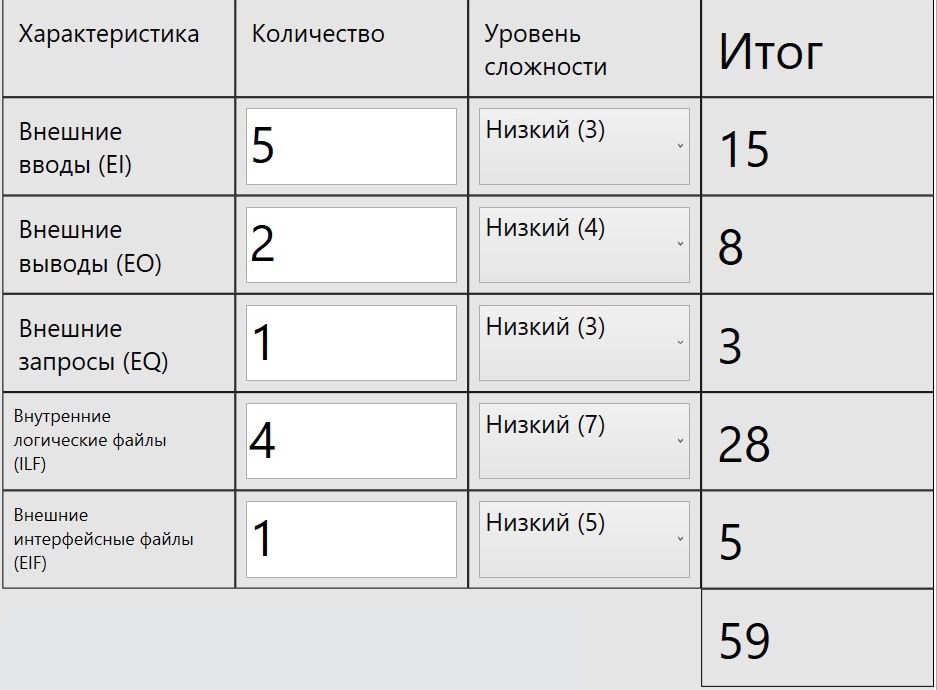
\includegraphics[scale=0.5]{nenorm.jpg}
\end{figure}

Зададим характеристики продукта:

Разработанное ПО состоит из трех компонентов. Первый компонент составляет по объему примерно 15\% программного кода и будет написан на SQL, второй (около 60\% кода) - на С\#, а третий в объеме 25\% кода - на Java.

 
\begin{itemize}
\item Обмен данными - 5.
\item Распределенная обработка-5
\item Производительность -3
\item Эксплуатационные ограничения по аппаратным ресурсам–2
\item Транзакционная нагрузка–3
\item Интенсивность взаимодействия с пользователем (оперативный ввод данных) – 4
\item Эргономические характеристики, влияющие на эффективность работы конечных пользователей - 1
\item Оперативное обновление–4
\item Сложность обработки–4
\item Повторное использование – 0 
\item Легкость инсталляции – 1
\item Легкость эксплуатации/администрирования – 2 
\item Портируемость – 2
\item Гибкость- 2
\end{itemize}

И тогда,

 \begin{figure}[H]
  \centering
  \caption{Нормированное количество функциональных точек. }
  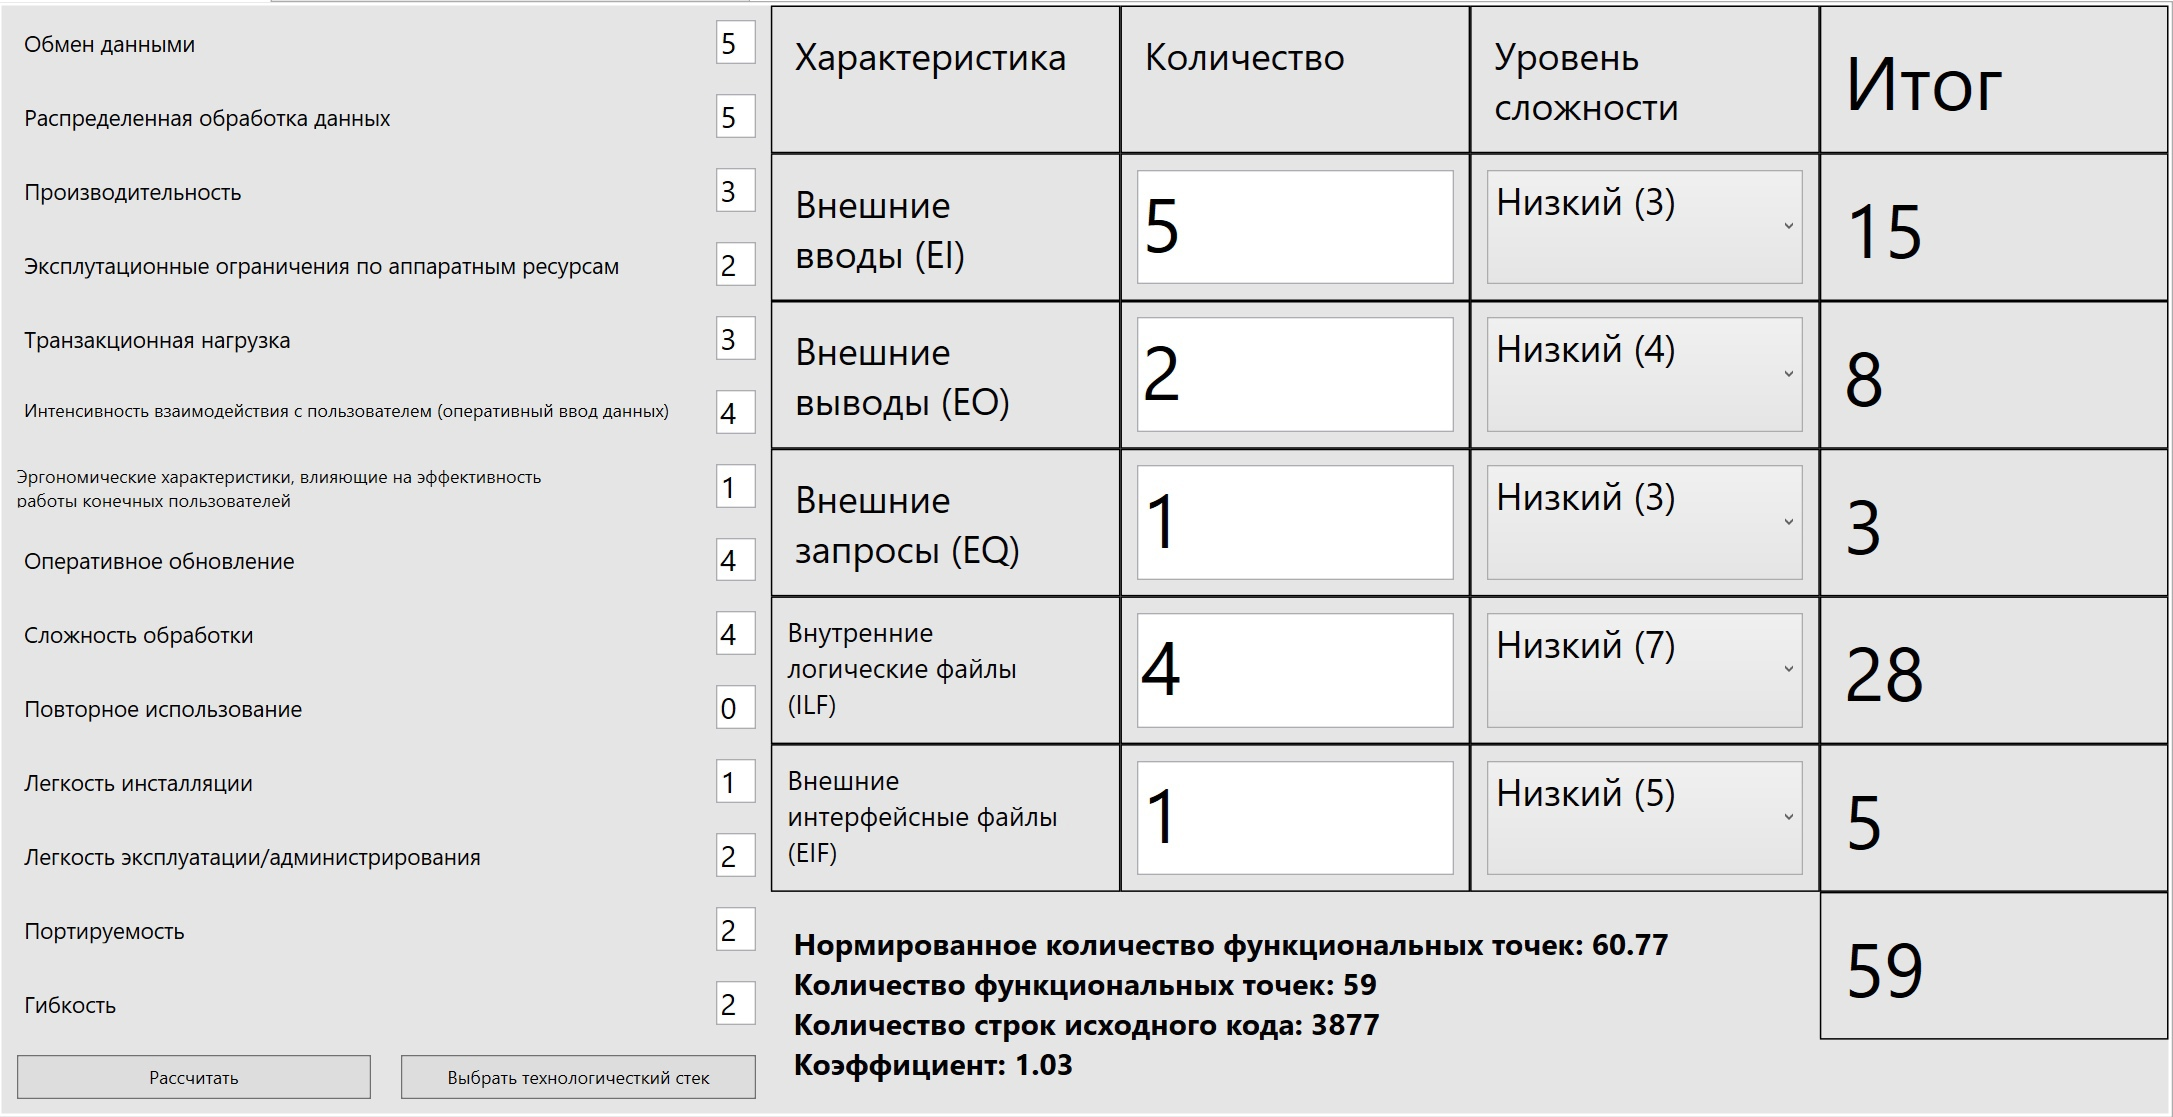
\includegraphics[scale=0.25]{norm.jpg}
\end{figure}

\item \textbf{Произвести оценку трудозатрат и длительности разработки по методике COCOMO II с использованием модели композиции приложения.}

Для реализации проекта была сформирована новая команда разработчиков, у отдельных членов которой имеется некоторый опыт создания систем подобного типа. В целях сплочения команды были проведены определенные мероприятия, что обеспечило на старте проекта приемлемую коммуникацию внутри коллектива. Заказчик не настаивает на жесткой регламентации процесса, однако график реализации проекта довольно жесткий. Несмотря на то, что предметная область является для разработчиков относительно новой, анализу архитектурных рисков было уделено лишь некоторое внимание. Организация только начинает внедрять методы управления проектами и формальные методы оценки качества процесса разработки.

Определим показатели проекта:

\begin{itemize}
\item Новизна проекта -- Почти полное отсутствие прецедентов, в значительной мере непредсказуемый проект (у некоторых членов команды имеется некоторый опыт создания подобных систем)
\item Гибкость процесса разработки -- Большей частью согласованный процесс (график жесткий, но точной регламентации нет)
\item Разрешение рисков в архитектуре системы -- Некоторое
\item Сплоченность команды -- Некоторая согласованность (благодаря мероприятиям, но команда все равно новая)
\item Уровень зрелости процесса разработки -- Уровень 1+ (только начинают внедрять)
\end{itemize}

\begin{figure}[H]
  \centering
  \caption{Факторы, влияющие на показатель степени в модели. }
  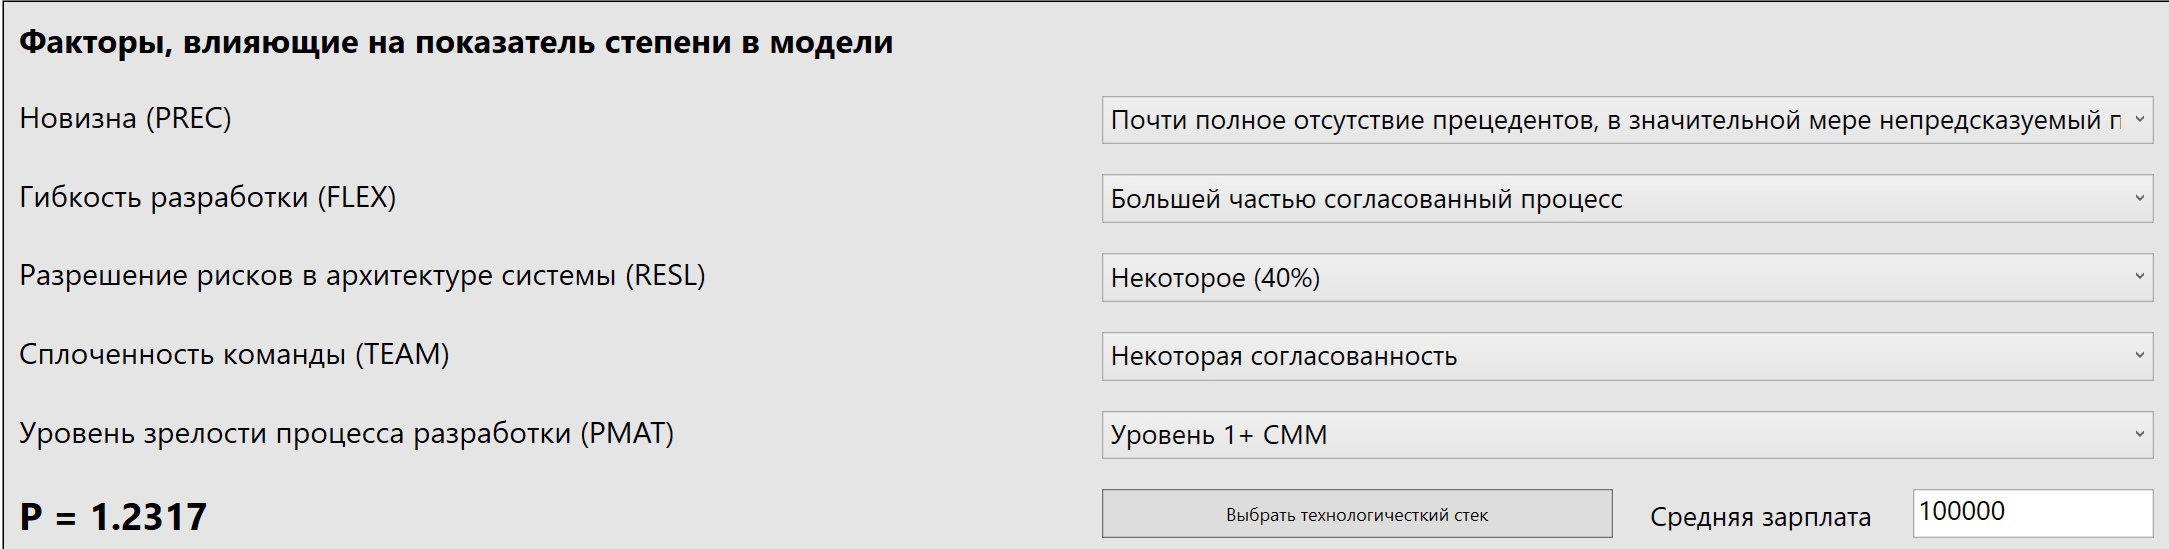
\includegraphics[scale=0.25]{factors.jpg}
\end{figure}

Повторное использование -- 0\%.

Опытность команды -- Низкая.

\textbf{Объектные точки.}

Рассмотрим каждую из страниц:
\begin{itemize}
\item Страница авторизации -- 3 простых поля и 1 средней сложности (обращение к бд)
\item Страница биржевых сводок -- 3 простых поля и 1 средней сложности (обращение к бд)
\item Страница заявок -- 1 простое поле и 2 средней сложности (обращение к бд)
\item Страница новой заявки -- 4 простых поля и 1 средней сложности (обращение к бд)
\end{itemize}

Также есть 2 модуля написанные на языках третьего поколения.

 \begin{figure}[H]
  \centering
  \caption{Время и трудозатраты по методике COCOMO II с использованием модели композиции приложения. }
  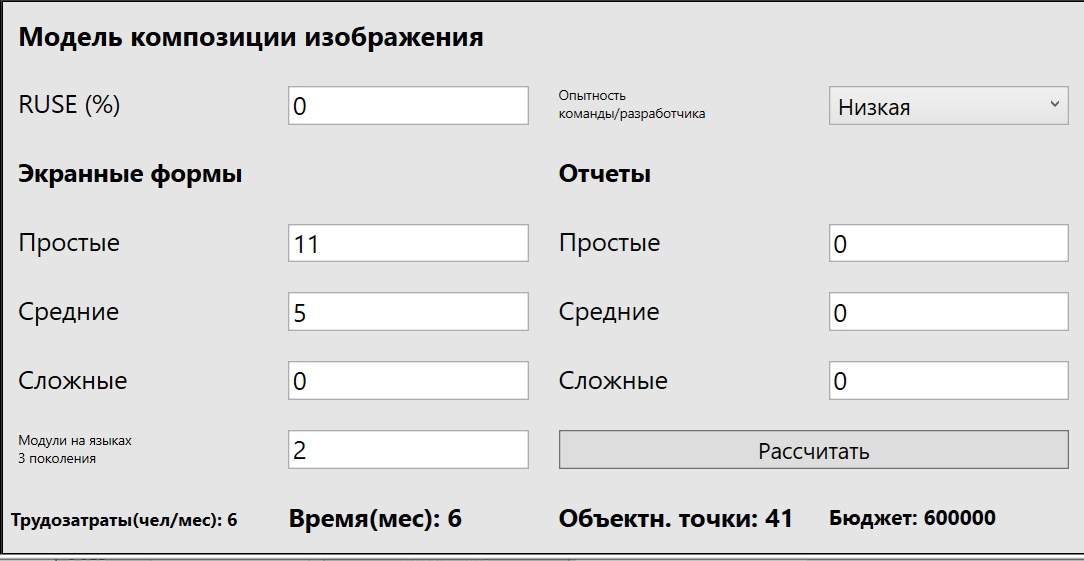
\includegraphics[scale=0.45]{compose.jpg}
\end{figure}


\item \textbf{Произвести оценку трудозатрат и длительности разработки по методике COCOMO II с использованием модели ранней разработки архитектуры.}

PERS -- номинальный

RCPX -- очень высокий

RUSE -- низкий

PDIF -- высокий

PREX -- низкий

FCIL -- очень высокий

SCED -- очень высокий

KSLOC примерно 4, из метода функциональных точек

 \begin{figure}[H]
  \centering
  \caption{Время и трудозатраты по методике COCOMO II с использованием модели ранней разработки архитектуры. }
  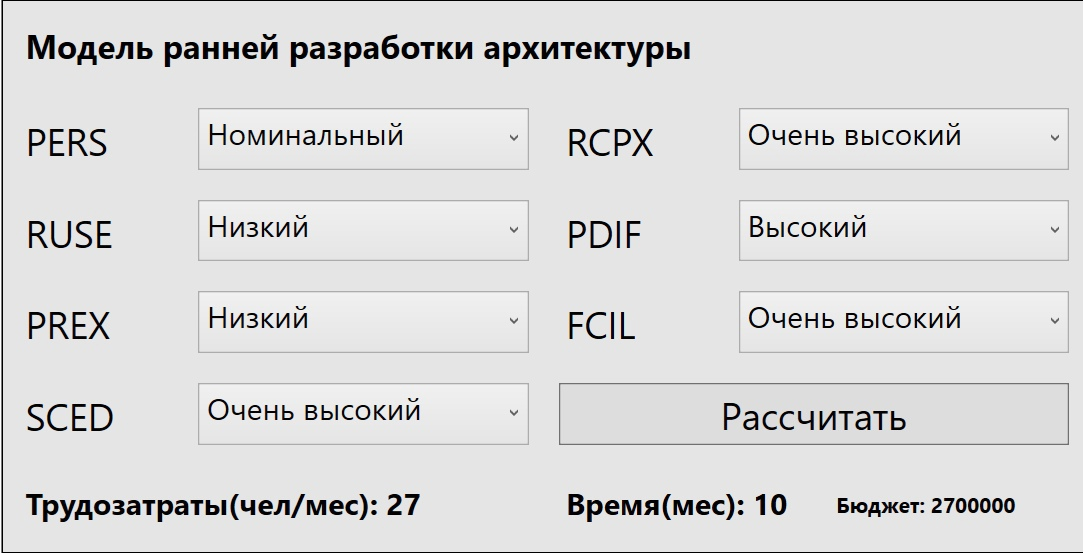
\includegraphics[scale=0.4]{early.jpg}
\end{figure}

\item \textbf{Вывод.}

В отличие от COCOMO учитывает больше человечески факторов: сплоченность, вовлеченность заказчика. Так же учитывается множество системных параметров и функциональных точек, каждая из которых отвечает за свой набор действий.

Так что модель позволяет оценивать разнообразные проекты, от начальных до крупных, от начинающих команд до опытных разработчиков. И для каждой найдутся свои параметры для расчетов.

\end{enumerate}

\end{document}